\chapter{Research}\label{research}
%TODO Mention RQ, problem statement
The aim of this paper is to examine the effect of reducing the dimensionality of the state-space in reinforcement learning (RL). In this section we will discuss the our research and its results. We will start by detailing our method in section \ref{research-method}; here we will explain the environments we used for our experiments, as well as the experiments that we ran. After this, we will show and discuss the results from these experiments in section \ref{research-results}. The discussion of the results will include an examination of how the different state-space reduction methods led to their results.

\section{Method}\label{research-method}
In this section we will explain our method: how we researched the effect of state-space dimensionality reduction on an RL agent. First, in section \ref{research-exp}, we will explain the experiments in general: the different agent setups that we compared. Then, we will look at the environments in which we ran the experiments in sections \ref{research-env-pysc2} and \ref{research-env-pong}, including their specific agent architectures.

\subsection{Experiments}\label{research-exp}
To examine the effect of the different dimensionality reduction methods, we implemented multiple RL agents using different reduction methods and compared their performance in two environments. In this section we will discuss the agents that we used. We will give a general overview here, and give more details about the architectures of the agents in the sections explaining the used environments: sections \ref{research-env-pysc2} and \ref{research-env-pong}.

The first agent mentioned is the baseline agent, which does not use a dimensionality reduction method, therefore using the full dimensions of the observation received from the environment. All other agents reduce the dimensionality of the observations, thus using less features.

Furthermore, to allow for a fair comparison of their performance, all agents must share as many architectural design choices and hyperparameter settings as possible. This is done by extending the baseline agent in all other agents. 

\noindent \textbf{Baseline agent}\newline
\noindent The baseline agent is a standard RL agent that does not use any dimensionality reduction. This is the agent that is extended by all other agents. It uses a DDQN strategy, as explained in section \ref{pl-dqn}. 

First, the agent receives an observation from the environment. This observation is passed to its neural network approximating the Q-function: its policy network. This returns a valuation for each action taken in this state. Then, the agent either chooses the action with the best valuation (i.e. acting greedily) or chooses a random action. Then, the chosen action is performed and we repeat this cycle until the end of the episode, whilst often training the policy network on stored transitions.

\noindent \textbf{PCA agent}\newline
\noindent The PCA agent uses PCA to reduce the dimensionality of the state observations. As mentioned, this is done by extending the baseline agent: after receiving an observation from the environment, the observation is processed by a PCA component lowering the observation dimensionality. This latent representation is then used by the agent as if it is the actual observations. This means that it is passed to the policy network to give an action valuation, as well as being stored in transitions used to train the network.

The PCA component is trained separately before being used by the agent. This is done by training the PCA on previously stored observations. It is important that these observations give a good representation of the entire environment to get a well trained PCA component.

\noindent \textbf{Pre-trained autoencoder agent}\newline
\noindent This agent is very similar to the PCA agent, except instead of using a PCA component, we are using an autoencoder to reduce dimensionality. Just like the PCA component, the autoencoder is pre-trained on stored observations. After this it is used by the agent to reduce the dimensionality of the observation. 

The autoencoder is trained by passing batches of observations to the encoder, which performs the dimensionality reduction. Its output is then passed to the decoder which tries to reconstruct the original data. The loss is then calculated by how similar the decoder output is, compared to the original data. Specifically, the \emph{mean squared error} is used.

When being used by an agent to reduce the dimensionality of an observation, only the encoder part of the autoencoder is used. When we speak of the output of the autoencoder in the context of being used by an agent, we mean the output of the encoder part. The autoencoder is not being trained further while in use by an agent. \newline

\noindent \textbf{\todo{I guess "online" is not strictly correct}Online trained autoencoder agent}\newline
\noindent  This agent is very similar to the pre-trained autoencoder agent. The only difference is the moment of training the autoencoder. In the pre-trained autoencoder agent, the autoencoder is trained before being used by an agent, using previously stored observations. In this online trained autoencoder agent, we are using an autoencoder that has not been pre-trained; it is being trained while being used by the agent. 

In this case, the agent itself still only uses the encoder part of the autoencoder. However, we now also store batches of observations and pass these to the training method of the autoencoder. This training method is the same as before: passing the observations to the encoder, whose output is passed to the decoder, whose output is compared to the original observation to calculate the loss and train the network.\newline

\noindent \textbf{DeepMDP agent}\newline
\noindent Just like the online trained autoencoder agent, the DeepMDP agent is completely trained while being used by the agent. It also uses an encoder, which has the same design as the encoders of the autoencoders. Differently from the autoencoder though, this encoder is actually part of the agent's network; whereas the autoencoder is a separate network, the DeepMDP simply extends the network of the agent, thus training the policy network and encoder simultaneously. This is further explained in section \ref{pl-deepmdp}.

In figure ... it can be seen that the observation given by the environment goes directly into the policy network. However, in contrast with the baseline agent, the observation first goes through the encoder, before going into the network representing the Q-function.

Another difference with the baseline agent is not shown in the figure: the DeepMDP makes use of an auxiliary objective to calculate the loss while training the policy network: the transition loss. This is also explained in section \ref{pl-deepmdp}.

\subsection{Environment: Starcraft II}\label{research-env-pysc2}
For our experiments we used the \emph{StarCraft II} environment by \emph{Blizzard}\cite{blizzard}. StarCraft II is a real-time strategy game, which has been used in RL research after the introduction of a learning environment created in collaboration with \emph{DeepMind}, called \emph{SC2LE} and a corresponding Python component called \emph{PySC2}\cite{pysc2}.

In particular we are using a PySC2 minigame called \emph{MoveToBeacon}. This minigame simplifies the StarCraft II game. Here, the RL agent must select an army unit and move it to a given beacon. To simplify our RL agent, selecting the army unit is implemented as a script, thereby focusing our research on moving the army unit to the beacon. A screenshot of the game is given in figure \ref{fig:pysc2_SS}. 

\begin{figure}[h]
    \centering
    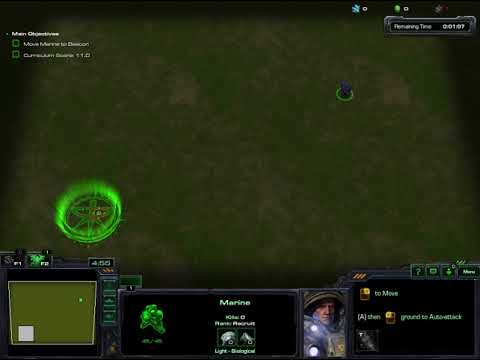
\includegraphics[width=0.75\textwidth]{pysc2_SS}
    \caption{Screenshot of the minigame \emph{MoveToBeacon} in \emph{StarCraft II}.}
    \label{fig:pysc2_SS}
\end{figure}

An \textbf{observation} received by the agent in this minigame is given by a $32 \times 32$ grid, representing the entire state of the game, \todo{Is this correct? Or are there actually perhaps only 3 features or something?} giving a total of \textbf{$1024$ features}. Each cell in the grid represents a tile in the game. It can have one of three values: a 0 denoting an empty tile, a 1 denoting the army unit controlled by the agent, or a 5 denoting the beacon. The beacon comprises more than one tile, namely a total of $21$ tiles; it comprises five adjecent rows, where the first comprises three adjecent columns, followed by three rows of five columns, followed by a row of three columns. Because of this, the beacon has $27 \cdot 27$ places where it could be, with the army unit having $1003$ tiles left to be. This gives \todo{Is this a correct usage of state-space?} a total state-space of $32 \times 32$ with a cardinality of $27 \cdot 27 \cdot 1003 = 731.187$. An example of such a state observation can be seen in figure \ref{fig:state_example}.

\begin{figure}[h]
    \centering
    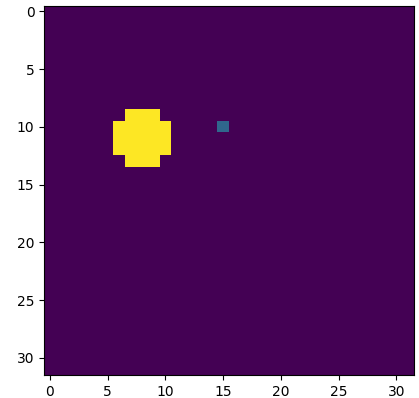
\includegraphics[width=0.75\textwidth]{AE_State_original}
    \caption{A state observation received by the RL agent, for the StarCraft II minigame MoveToBeacon. The yellow cells represent one beacon; the blue cell represents the army unit controlled by the player; all other cells are empty.}
    \label{fig:state_example}
\end{figure}

An \textbf{action} taken by the agent is given by an $(x,y)$ coordinate with $x,y \in \{0 .. 31\}$. This denotes the (indices of the) cell in the grid that the army unit will move to. Each action sent to the environment will result in $8$ in-game steps, meaning that if the given coordinates are further away than 8 steps, the unit will only walk 8 steps towards the given coordinates before the agent has to choose a new action.

Lastly, an \textbf{episode} takes $120$ seconds. The goal is to move the army unit to the beacon as often as possible in this time limit, each time adding $1$ point to the episode score. At the start of each episode, the beacon and army unit are placed randomly. Whenever the army unit reaches the beacon, only the beacon will be relocated randomly. 

Within the $120$s time limit, the agent will be able to take 239 steps/actions. An agent following a random policy gets a score of about $0-3$ points per episode (again, one point for each time the army unit reaches the beacon), whereas a scripted agent scores about $25-30$ points per episode (meaning the agent on average needs $8$ or $9$ actions before reaching a beacon).

\subsubsection{Agents setup}
We will now explain the architectures of the agents used in the Starcraft II environment. We will only give a general overview, referring to appendix \ref{appendix} section \ref{appendix-agents} for details on the neural network architectures and hyperparameter settings. 

Whereas the baseline agent uses the $32 \times 32$ observations given by the environment, all other agents reduce the dimensionality to $16 \times 16$. This means that the number of features in an observation are reduced from \todo{Again, is this correct?}$1024$ to $256$.

Though the baseline agent's architecture is extended by all other agents (in order to keep the agents as similar as possible), one important change must be made. The policy networks of all agents are convolutional neural networks, and the output dimensions of a convolutional layer depends on the dimensions of its input. The baseline agent's policy network receives a $32 \times 32$ input, whereas the other agents receive a $16 \times 16$ input. In all cases, the output dimensions must be $32 \times 32$. This is because the network approximates the Q-function: a valuation of all actions for a given state. Since an action in our environment is defined by the coordinates the army unit must walk to, there are $32 \times 32$ possible actions. To deal with this difference in input dimensions, the first layer of the policy networks of the non-baseline agents are modified (using different stride and padding sizes) to increase the dimensionality to $32 \times 32$.\newline

\noindent \textbf{Baseline agent}\newline
\noindent The baseline agent is a standard RL agent that does not use any dimensionality reduction and is extended by the other agents.

Its policy network consists of three convolutional layers: the first layer being a transposed convolutional layer \cite{transpose}, the other two being regular convolutional layers. The use of the transposed convolutional layer allows for the possibility of upsampling the dimensionality of the given input. This is needed in agents using dimensionality reduction, where the input for the network is $16 \times 16$, but the output needs to be $32 \times 32$ to cover the action space. However, for our baseline agent, the input dimensions, $32 \times 32$, must remain the same, which is achieved by setting the stride of the first layer to $1$. This way, both the dimensions of the input and the output of the network are $32 \times 32$ (where its input represents the current state observation and its output the action valuation).\newline

\noindent \textbf{PCA agent}\newline
\noindent The PCA agent uses PCA to reduce the dimensionality of the state observations from $32 \times 32$ to $16 \times 16$. To do this, the observation input must first be flattened, and its output must be reshaped to $16 \times 16$.

The output of the policy network representing the Q-function must remain $32 \times 32$, since we have $32 \cdot 32$ possible actions: one action per coordinate. Therefore, the first layer in the policy network, the aforementioned transposed convolutional layer, has a stride of $2$ and an output padding of $1$. This changes the dimensions from $16 \times 16$ to $32 \times 32$. 

The PCA component is trained on $240.000$ previously stored observations, which corresponds to observations from $1000$ episodes. These have been gathered using a scripted agent. The first $256$ principal components in our PCA (representing a $16 \times 16$ dimensional observation), contain roughly $96\%$ of the variance of the original data. We are using a scalar to standardize the observation data as explained in section \ref{pl-pca}. \newline

\noindent \textbf{Pre-trained autoencoder agent}\newline
\noindent Just like the PCA component, the autoencoder is pre-trained on the same $240.000$ observations. After this its encoder is used by the agent to reduce the dimensionality of the observation. 

The encoder and decoder of the autoencoder are convolutional neural networks. The encoder uses two convolutional layers: the first has a stride of $2$, which reduces the dimension to $16 \times 16$. The decoder, which tries to reconstruct the original data, uses three convolutional layers. The first layer is a transposed convolutional layer with a stride of $2$, to bring the dimensions back to $32 \times 32$. The other two layers are regular convolutional layers. 
 
\noindent \textbf{\todo{I guess "online" is not strictly correct}Online trained autoencoder agent}\newline
\noindent  This agent has the exact same design as the pre-trained autoencoder agent. As mentioned, the only difference is the moment of training the autoencoder: instead of training on previously stored observations, we are now training the autoencoder simultaneously with the RL agent.

\noindent \textbf{DeepMDP agent}\newline
\noindent The encoder of the DeepMDP has the same design as the encoders of the autoencoders: one convolutional layer with stride $2$ to reduce dimensions and a second convolutional layer with stride $1$. 

The auxiliary objective to calculate the transition loss represents the cost of all possible transitions from a given latent representation. This means that its output has dimensions $(32 \times 32) \times 16 \times 16$. The tuple $(32, 32)$ represents the actions that can be taken in the current state, while the other two dimensions, $16 \times 16$ represent the next (predicted) latent observation. It has only one layer, a convolutional layer, with $32 \times 32$ output channels to represent the action dimensions.

\section{Results}\label{research-results}
In this section we will show and discuss the results from the experiments mentioned in section \ref{research-exp}. We start by discussing the general results of the agents in section \ref{research-general-results}, and then discussing and interpreting these results in section \ref{research-discussion}.

\subsection{Research results}\label{research-general-results}
The results from running the different agents in the Starcraft II minigame MoveToBeacon, can be seen in figure \ref{fig:results-agents}. For each agent, the score, i.e. reward, per episode is shown, as well as an average score per $30$ episodes. Again, a scripted agents scores around $25-30$ per episode, and an agent following a random policy around $0-3$.


\begin{figure}[h]
	\centering
	\begin{subfigure}[b]{0.75\textwidth}
		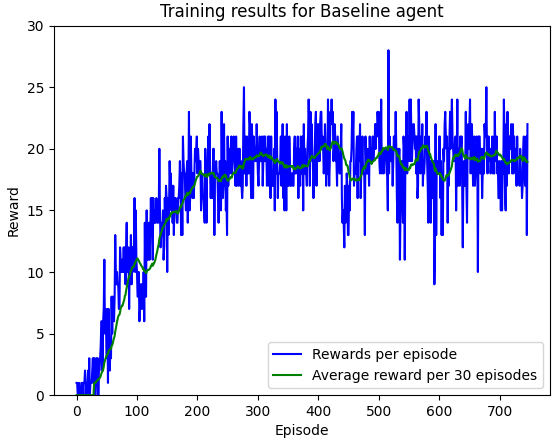
\includegraphics[width=0.75\linewidth]{Base_agent_results}
		\caption{Results for the baseline agent.}
		\label{fig:results-base} 
	\end{subfigure}
	\begin{subfigure}[b]{0.75\textwidth}
		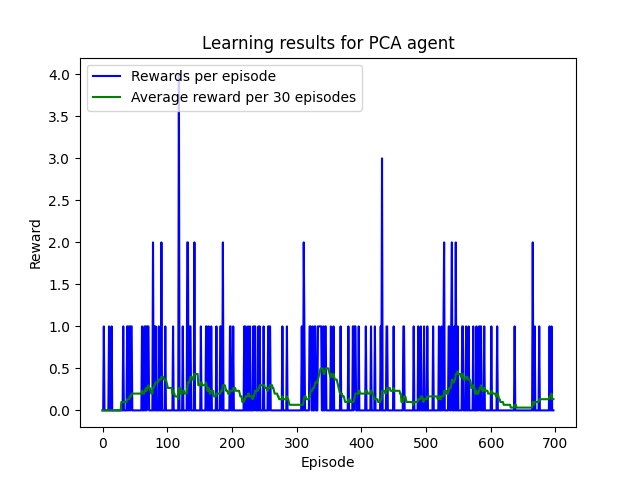
\includegraphics[width=0.75\linewidth]{PCA_with_scalar_agent_results}
		\caption{Results for the PCA agent using a scalar.}
		\label{fig:results-pca}
	\end{subfigure}
	\begin{subfigure}[b]{0.75\textwidth}
		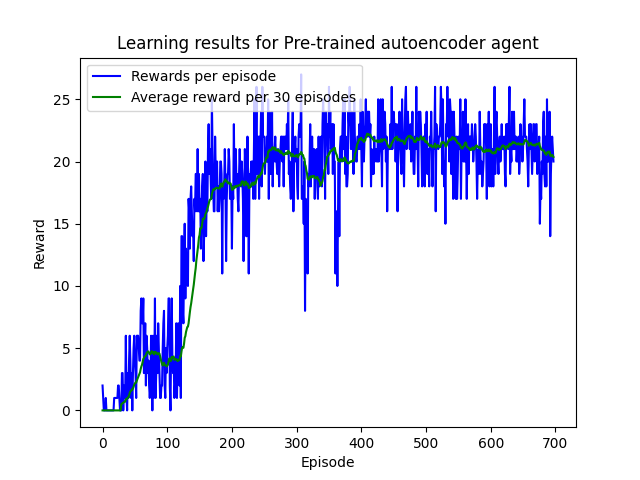
\includegraphics[width=0.75\linewidth]{Pretrained_autoencoder_agent_results}
		\caption{Results for the pre-trained autoencoder agent.}
		\label{fig:results-ae}
	\end{subfigure}
	\caption{Results of the different RL agents.}
\end{figure}%	
\begin{figure}[ht]\ContinuedFloat
	\begin{subfigure}[b]{0.75\textwidth}
		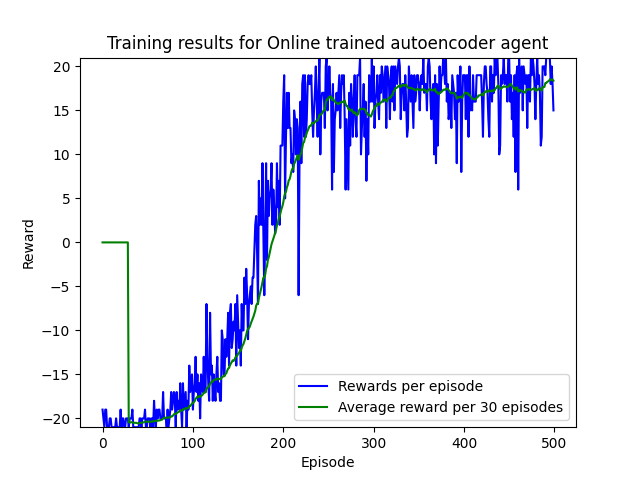
\includegraphics[width=0.75\linewidth]{Online_autoencoder_agent_results}
		\caption{Results for the online trained autoencoder agent.}
		\label{fig:results-online-ae}
	\end{subfigure}
	\begin{subfigure}[b]{0.75\textwidth}
		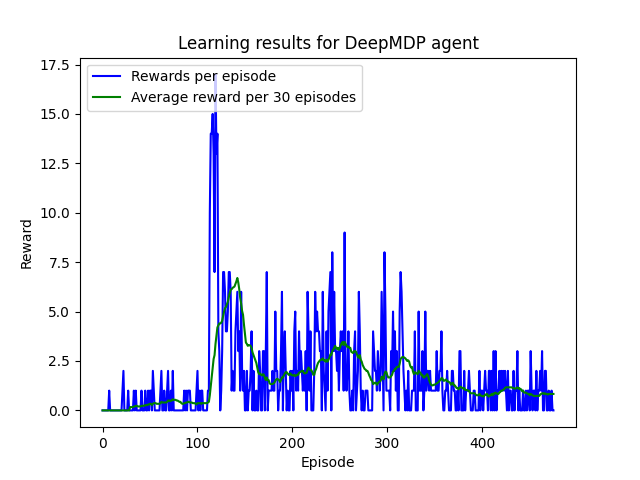
\includegraphics[width=0.75\linewidth]{Deepmdp_agent_results}
		\caption{Results for the DeepMDP agent.}
		\label{fig:results-deepmdp}
	\end{subfigure}
	\caption{Results of the different RL agents(cont.).}
	\label{fig:results-agents}
\end{figure}

As can be seen in subfigure \ref{fig:results-base}, the baseline agent converges to a policy scoring around $19$ per episode. This policy is reached after roughly $600$ episodes. Already after episode $300$ does it oscillate around scoring $17-20$ while also sometimes having an episode score of around $10$. After this it still needs another $300$ episodes to get to a more consistent policy.

The results for the PCA agent can be seen in figure \ref{fig:results-pca}. Though this shows the results for the agent using a PCA with a scalar, similar results were achieved without using a scalar. Furthermore, no matter what neural network architecture used in the agent (having used multiple different linear network architectures and different CNN architectures), it always remained at a policy performing at the level of a random policy, i.e. scoring around $0-3$ per episode.

The results for the agent using a pre-trained autoencoder, in figure \ref{fig:results-ae}, show that this agent preforms a little better. Not only does it converge to a slightly better policy scoring around $21$ per episode, it also converges quicker; it is already consistent after roughly $400$ episode, instead of $600$. 

We also show the results of training the autoencoder itself. As mentioned, it is trained on $240.000$ observations, corresponding to $1000$ episodes. Whereas each agent's training (except for the DeepMDP) took roughly $90$ minutes, training the autoencoder itself on $1000$ episodes worth of observations only took about $2.5$ minutes. The loss history for the autoencoder can be seen in figure \ref{fig:ae-loss}. After roughly $6000 \cdot 25 = 150.000$ observation it converges to its final loss.

\begin{figure}[h]
    \centering
    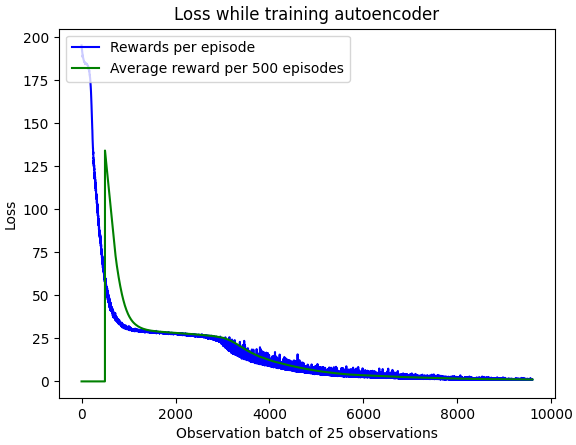
\includegraphics[width=1\textwidth]{ae_loss}
    \caption{Losses per 25 observations for training the autoencoder on $240.000$ state observations.}
    \label{fig:ae-loss}
\end{figure}

Compared to the pre-trained autoencoder agent, the agent using an untrained autoencoder that is being trained while the agent is trained, performs a little worse. It converges after roughly $500$ episodes to a policy around $19-21$. Not only does it take longer to converge and converges to a slightly worse policy, it is also less consistent. Even after $400$ it still has episodes scoring around $13$. This shows it is less consistent than its pre-trained counterpart.

Lastly we have the DeepMDP agent. After $130$ episodes, this agent suddenly jumps up from a random policy to scoring around $15$. However, after several episodes it starts going back down, alternating between scoring at a random policy and scoring around $7$, until finally reaching a random policy again. Furthermore it takes a lot longer to train. For the other agents, each episode took only a few seconds, whereas each episode in the DeepMDP agent takes $2.5$ minutes.

\subsection{Discussion}\label{research-discussion}
The first notable results is the PCA agent giving a policy that remains at a policy at the level of a random policy during its $800$ episode training, therewith performing way worse than the other agents. A possible explanation might be that the PCA reduction loses (too much) spatial information. \todo{Citing}Although PCA can be used for image compression, where spatial information is retained, it is a lot more lossy than for instance an autoencoder.

Figure \ref{fig:pca-state} shows an example of the PCA transformation on an observation. figure \ref{fig:pca-original} shows the original observation that the agent would get from the environment. Figure \ref{fig:pca-latent} shows the latent representation after using PCA for dimensionality reduction. as mentioned before, this uses $256$ principal components, capturing roughly $96\%$ of the original data. Here we can see that no spatial information is retained, making it impossible for the agent to train a meaningful policy on. 

Furthermore, we also tested a different PCA setup where we used all $1024$ principal components. Here, we again fitted the PCA on the same observations but keeping all principal components, giving a new $32 \times 32$ observation (and therefore not doing any dimensionality reduction). Transformation of an observation gave similar results: spatial information was lost. The problem therefore lies in the fitting process. A possible explanation for the bad transformation performance, might be that a single observation is very sparse. Even though the PCA is fitted on $240.000$ observations, each single observation is very sparse and at the same time, there are a lot of different possible observations due to the large state-space (see section \ref{research-env}). This combination might lead to the PCA not being able to generalize well enough. 

\begin{figure}[h]
	\centering
	\begin{subfigure}[b]{0.75\textwidth}
		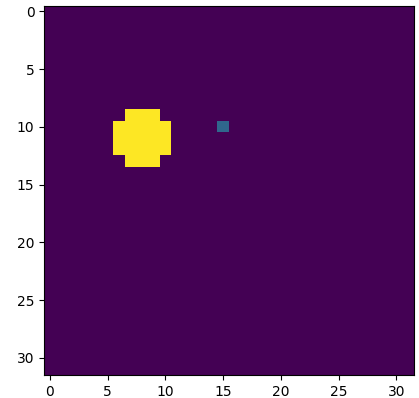
\includegraphics[width=0.75\linewidth]{AE_State_original}
		\caption{The original observation, i.e. the input for the PCA transformation.}
		\label{fig:pca-original} 
	\end{subfigure}
	\begin{subfigure}[b]{0.75\textwidth}
		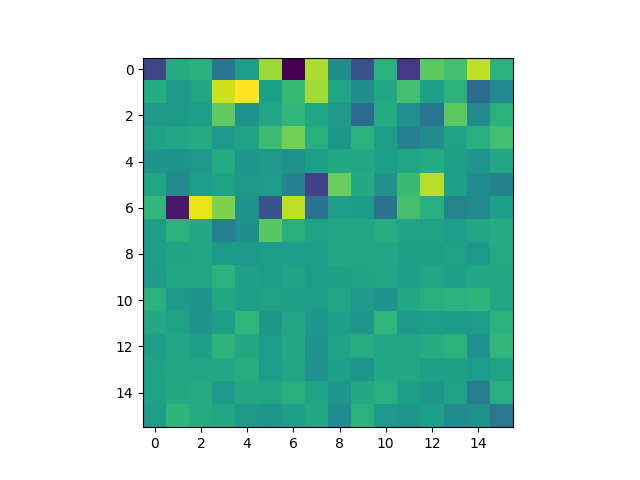
\includegraphics[width=0.75\linewidth]{pca_with_scalar_latent_state}
		\caption{The latent representation given by the PCA transformation}
		\label{fig:pca-latent}
	\end{subfigure}
	\caption{Latent representation and reconstruction of a state observation using PCA.}
	\label{fig:pca-state}
\end{figure}

Another interesting result is the performance of the pre-trained autoencoder agent. Not only does it match the baseline agent's performance, it even slightly surpasses it: it finds a slightly better policy (scoring around $21$ per episode on average, versus $19$), and more quickly converges to a consistent policy (after $400$ episodes versus $600$). Its better performance is despite the agent using imperfect information, while the baseline agent uses complete information.

Its performance is highly dependent on the quality of the output of the autoencoder. To get an understanding of why this agent achieves such good results, we will now examine the autoencoder in detail. Firstly, a correlation matrix is given in figure \ref{fig:ae-corr}. Based on $60.000$ state observations, it shows the correlation between the features of the original state observations (i.e. the input for the autoencoder) and the reduced state observations (i.e. the output of the autoencoder). The original data has dimensions of $32 \times 32$, whereas the reduced data has dimensions of $16 \times 16$, resulting in $1024$ and $246$ features respectively. Dark/black and light/beige colouring mean a high correlation (negative and positive correlation respectively), whereas a red colouring means no correlation and the white space means there was to too little variance to calculate a correlation. The latter case simply follows from the beacon and army unit not visiting these parts of the map enough times during the used episode observations.

What can be seen from this matrix, is that each cell in the reduced data grid, correlates to a block (a few adjacent rows and columns) of cells of the original data grid. This explanation can be abducted from each feature of the reduced data being highly correlated to a few features of the original data, then being uncorrelated for $32$ features, after which highly correlated features are found again. This jump of $32$ features corresponds to a jump of one row in the original data grid. Thus, a reduced feature correlates to a block of the original features.

\begin{figure}
	\centering
	\makebox[0pt]{%
	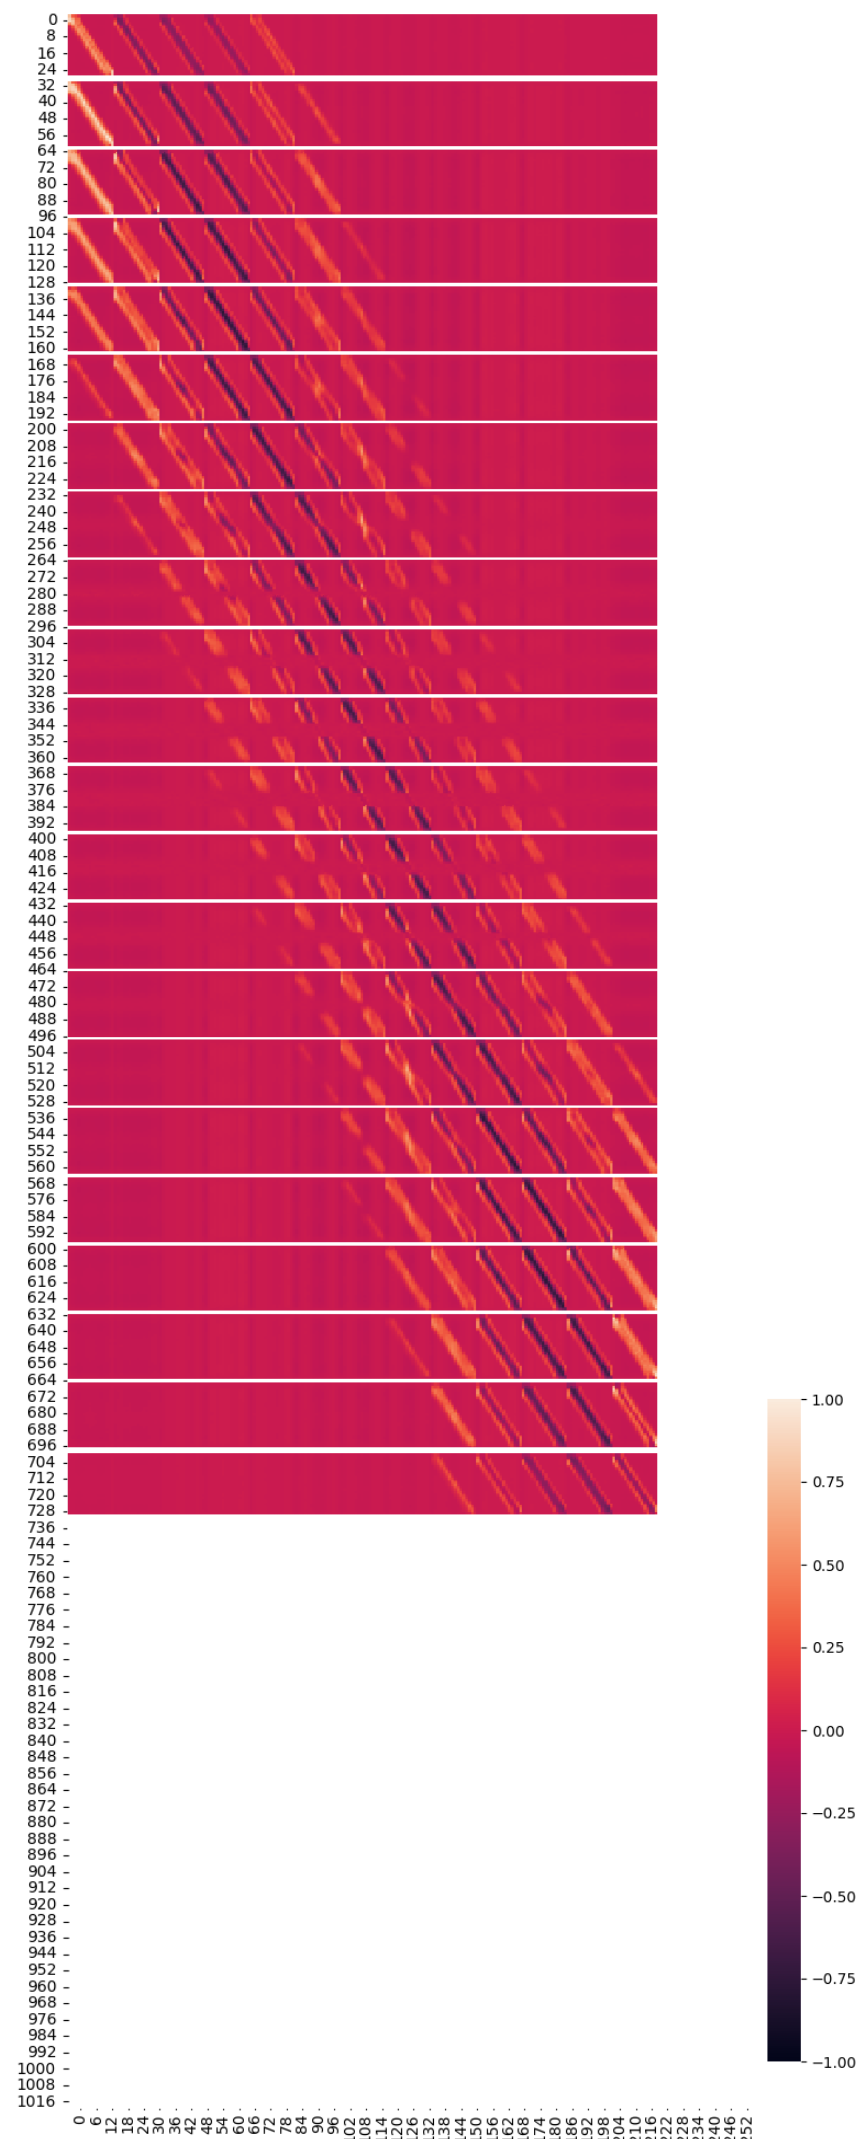
\includegraphics[width=1.0\paperwidth]{AE_corr_matrix_cropped}}
	\caption{Correlation matrix for the autoencoder used in the pre-trained autoencoder agent, based on $60.000$ state observations. The x-axis contains the features of the original observations, and the y-axis contains the features of the reduced state observations.}
	\label{fig:ae-corr}
\end{figure}

We also show the feature map visualisation for the enoder of the autoencoder in figure \ref{fig:ae-featuremap}. This shows the output of each channel in each convolutional layer of the encoder of the autoencoder. The original $32 \times 32$ input for the encoder is given in figure \ref{fig:ae-featuremap-original}. Like before, the yellow octagon is the beacon, the blue square is the army unit controlled by the agent, and purple parts are the empty tiles. The feature map for the first convolutional layer is given in figure \ref{fig:ae-featuremap-layer1}. It shows the output of its $32$ channels, each having a dimensionality of $16 \times 16$. What can be seen here is that each channel seems to pay attention to a different part of the observation, sometimes putting more emphasis on the empty cells, sometimes more on a certain side of the beacon and/or the army unit. Lastly the feature map of the second layer is given in figure \ref{fig:ae-featuremap-layer2}. Since this has only one channel, this also corresponds to the output of the encoder. 


\begin{figure}[h]
	\centering
	\begin{subfigure}[b]{1\textwidth}
		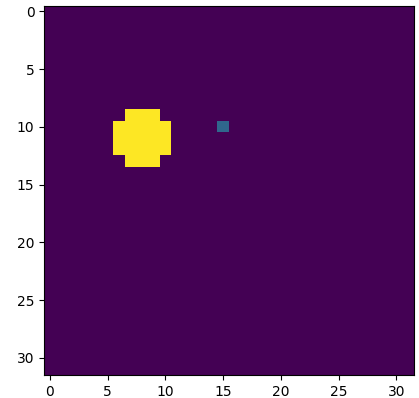
\includegraphics[width=1\linewidth]{AE_State_original}
		\caption{The original observation, i.e. the input for the autoencoder.}
		\label{fig:ae-featuremap-original} 
	\end{subfigure}
	\begin{subfigure}[b]{1\textwidth}
		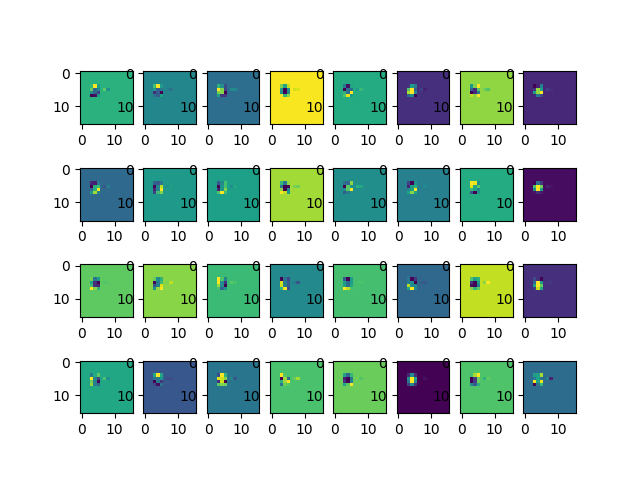
\includegraphics[width=1\linewidth]{AE_Layer_1_Feature_Map}
		\caption{The feauture map of the first convoluational layer, showing the output of its $32$ channels.}
		\label{fig:ae-featuremap-layer1}
	\end{subfigure}
	\caption{A feature map visualisation for the autoencoder used by the pre-trained autoencoder agent.}
\end{figure}%	
\begin{figure}[ht]\ContinuedFloat
	\begin{subfigure}[b]{1\textwidth}
		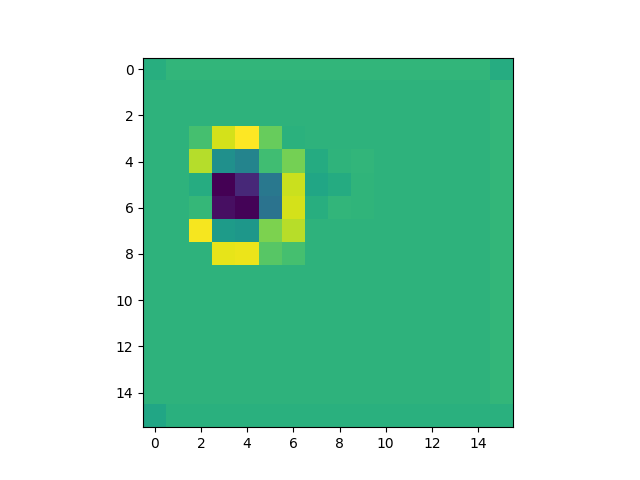
\includegraphics[width=1\linewidth]{AE_Layer_2_Feature_Map}
		\caption{The feature map of the second convolutional layer, showing the output of its single channel. Since it has only one channel, this also corresponds to the output of the autoencoder.}
		\label{fig:ae-featuremap-layer2}
	\end{subfigure}
	\caption{A feature map visualisation for the autoencoder used by the pre-trained autoencoder agent (cont.).}
	\label{fig:ae-featuremap}
\end{figure}

This autoencoder agent not only outperforms the baseline agent, it also (less surprisingly) outperforms the online trained autoencoder agent. This latter agent converges to a slightly worse policy and takes more episodes to get there, while remaining not very consistent (sometimes scoring only about $13$ points in an episode). This can of course be explained by the fact that this agent not only trains a policy network, but also, separately, the autoencoder. This means that for many episodes, the policy network is trained on a rather imperfect representation; the pre-trained autoencoder needed roughly $150.000$ observations before getting close to its final loss. Still, it got to a policy similar to the baseline agent (even scoring slightly better on average) in a similar number of episodes; the main difference being that the baseline agent is much more consistent. %TODO 180.000 beter bekijken, gegokt

Besides outperforming the online trained autoencoder agent, the pre-trained agent has another advantage. Since the autoencoder can be trained separately from the agent, we can reuse the autoencoder for different agents acting in the same environment. This allows for the possibility of training an autoencoder once, after which multiple agents can be trained on less features, allowing for less computation cost to train each agent. This is also substantiated by the autoencoder taking little time train.

Lastly, the DeepMDP performs horribly and something seems off with its implementation, since it goes to a decent policy scoring around $15$ per episode, then quickly dropping back to the level of a random policy. I'm not sure what is going wrong here. I did print out the loss during a few different moments in training. Its loss calculation consists of several different losses: firstly the usual DDQN loss calculated like in all other agents. Secondly, the loss of the auxiliary objective: the transition loss. Lastly we have the gradient penalty for each part of the network. All these losses are added together, with the sum of the gradient penalties being multiplied by $0.1$ (a hyperparameter).

After $133$ episodes, when the agent gets decent scores of around $15$ points per episode, the losses look as follows:
\begin{itemize}
\item DDQN Loss: 0.008
\item Transition Loss: 400
\item Encoder gradient penalty: 20
\item Policy gradient penalty: 20
\item Auxiliary objective gradient penalty: 3.5 million
\item Total loss: 38.000
\end{itemize}

A few episodes later, it goes down to a policy scoring about $0$ per episode:
\begin{itemize}
\item DDQN Loss: 0.002
\item Transition Loss: 1000
\item Encoder gradient penalty: 90
\item Policy gradient penalty: 90
\item Auxiliary objective gradient penalty: 1.5 million
\item Total loss: 16.000
\end{itemize}

After $248$ episodes, it is still at the level of a random policy:
\begin{itemize}
\item DDQN Loss: 0.0008 
\item Transition Loss: 22.000
\item Encoder gradient penalty: 3.5
\item Policy gradient penalty: 3.5
\item Auxiliary objective gradient penalty: 2000
\item Total loss: 22.000
\end{itemize}

We can see here that there is probably something off with the loss calculation, since they are extremely disproportional.
OR PERHAPS the problem lies in that there is no good prediction of transition (i.e. next state) possible due to the continuous random replacement of the beacon when following a good policy and therefore the only way to lower the transition loss (does this also entail the aux penalty?) would be to follow a policy that does not reach the beacon.